% Murmuration — IEEEtran journal draft (converted 2026-11-09; content = paper/main.md)
% Build: pdflatex main.tex (x2). Discussion via GitHub Issues on github.com/xuanjat/murmuration.
\documentclass[journal]{IEEEtran}
\usepackage{amssymb,amsmath}
\usepackage{graphicx}
\usepackage{url}
\usepackage[colorlinks=true,linkcolor=blue,citecolor=blue,urlcolor=blue,breaklinks=true]{hyperref}
\providecommand{\tightlist}{\setlength{\itemsep}{0pt}\setlength{\parskip}{0pt}}
\hyphenation{op-tical net-works semi-conduc-tor}

\begin{document}

\title{Murmuration: Federating LLM Agents Across Machines with Nothing but Text}

\author{Lifeng~Tian and Chengxu~Han\thanks{Corresponding author contact: \texttt{xuanjat77@gmail.com}; co-author: chengxuhan0313@163.com. Manuscript received November 2026. Source, artifacts, and discussion channel (GitHub Issues): \url{https://github.com/xuanjat/murmuration}}}

\markboth{Murmuration: Federating LLM Agents Across Machines with Nothing but Text}{}

\maketitle

\begin{abstract}
Personal LLM-agent harnesses now run simultaneously on many heterogeneous machines (workstations, cloud servers, LAN boxes, offline nodes), yet each instance is a silo: its sessions, files, and learned lessons do not cross machine boundaries, and letting one agent operate another machine's shell is a security red line. We present \textbf{Murmuration}, a method framework that federates \emph{independent} agent instances through a single shared, plain-text context database, adding no broker or middleware beyond that store. Its core is a \textbf{semantic-level transport model}: messages carry only speech-act headers (five performatives), wire-level identities, and wall-clock timestamps; anything larger than a small threshold travels as a \textbf{content-addressed pointer} (path + SHA-256 + byte count) that is verified \emph{outside} any agent's context window. We formalize a message calculus and derive three cost properties --- design invariants implied by the payload threshold and the manifest discipline, not independently established empirical results: per-delivery context cost scales with the pointer list rather than payload bytes, and drops to a constant header when the manifest itself travels as a file; novelty detection is O(1) via fixed-width timestamp comparison; and k-hop relay never re-pays payload context, since pointer forwarding and digest verification are idempotent. Around the transport we specify organizational governance: a versioned, incident-driven handbook with red lines, role-scoped acknowledgment obligations, and time-triggered watchkeeping suited to turn-based agents. We report a sanitized eleven-day (elapsed) field deployment across five heterogeneous machines (protocol v1.0→v1.4, eight role types, 45 cross-machine lessons, 13 archived incidents, deliveries of up to 1,300 files, each verified by per-file SHA-256 corruption checks) and a 49-system novelty assessment. Within the window the room carried 283 structured messages (mean 26/day, peak 49/day) --- 37 typed data deliveries, 29 asks, and 89 acknowledgment discharges --- with more than three thousand per-file SHA-256 checks at byte equality and zero mismatches; payload content (scientific-experiment pipelines, document drafting, paper writing) never enters this paper, only counts and shapes. A controlled same-window ablation (three rounds x six abstracted tasks, Latin-square order) corroborates the field evidence: the federation arm cut makespan by 34\% with three-times-lower variance, at $+1.3$ turns and $+57\%$ context bytes per task, with verification parity (18/18 first pass per arm). Per our search (2026-11), no public scheme combines all of: heterogeneous cross-machine instances, a shared plain-text context database as the sole substrate, versioned incident-driven handbook governance, pointer-based delivery-integrity checks, turn-driven watchkeeping, and field evidence; we state claims at a deliberately conservative level.
\end{abstract}

\begin{IEEEkeywords}
multi-agent systems, LLM agents, agent communication, semantic
communication, content addressing, coordination artifacts,
organizational governance, field deployment.
\end{IEEEkeywords}



\section{Introduction}


A single developer or small team today routinely operates several
LLM-agent instances {[}1{]}: one on a laptop, one on a cloud server, one
on a LAN machine without external network, and so on. Each instance is
\emph{turn-based} (it acts, returns, and is re-invoked),
\emph{context-bounded} (its working memory is a token window that is
billed and that degrades with length), and \emph{environment-privileged}
(it holds credentials and shell rights on exactly one machine). Three
consequences follow.

\begin{enumerate}
\def\labelenumi{\arabic{enumi}.}
\tightlist
\item
  \textbf{Silos.} Lessons learned on machine A (a command trap, a config
  pitfall, an incident root cause) are invisible to machine B unless a
  human copies them.
\item
  \textbf{Context scarcity as the true bandwidth.} When agents
  collaborate, the scarce channel is not network bandwidth but the
  context window {[}2,3,4{]}: every byte that enters it is paid for in
  tokens and competes with the task at hand.
\item
  \textbf{The remote-shell red line.} The naive fix --- letting agent A
  ssh into machine B and run commands --- merges trust domains and is
  exactly what operational red lines forbid (``never operate another
  machine on its behalf'').
\end{enumerate}

Existing answers address \emph{single-host} multi-agent work (built-in
agent teams, swarm frameworks, conversation orchestrators)
{[}5,6,7,8,9{]} or \emph{platform-scale} infrastructure and
cross-machine agent protocols (organization-level substrates with
identity, discovery, and container orchestration) {[}10,11{]}. Neither
fits the personal/small-team setting: independent heterogeneous
instances, no open ports, no broker clusters, no budget for platform
operations, and a human who must be able to audit everything by reading
plain text.

\textbf{Positioning as a research prototype.} Murmuration is a research
prototype for cross-architecture multi-agent collaboration and work
relay (cross-harness by design): independent agent instances on
different machine architectures --- and different builds of the DeepSeek
Harness (DSH) family {[}9{]} --- hand work to one another through the
federation, and compared with traditional single-session execution it
delivers the same class of multi-agent coordination at near-zero
marginal infrastructure cost in our deployment (no broker, no open
ports, no platform team). Concurrently, the DeepSeek Harness team's
Super-agent design exploration {[}12{]} reports the same attention
bottleneck --- a human sustains only 3--5 active sessions --- and
answers it inside one organization's footprint with a two-layer
Router/Worker architecture, event-driven triggers with thread
subscription, Inline \& Spill and Chain-of-Recall context mechanics,
speculative execution, and a Watchdog control loop, while listing
cross-instance agent-to-agent (A2A {[}10{]}) communication and
cross-session human collaboration as open problems. We occupy exactly
that open slot from the opposite direction: rather than redesigning the
interior of one agent stack, we federate already-deployed independent
instances with plain-text organizational artifacts --- nothing but text
in the coordination plane, since payload bytes move over pre-existing
point-to-point channels --- across machines and harness builds.

\textbf{Contributions.} (i) A method framework that federates
independent, heterogeneous LLM-agent instances over one shared
plain-text context database, adding \textbf{no broker or middleware
beyond that store} (§3). (ii) A \textbf{semantic-level transport model}
with a message calculus and three cost propositions (§4), positioned
against speech-act communication, tuple spaces, publish/subscribe with
consumer offsets, content addressing, and provenance standards. (iii) An
\textbf{organizational governance layer}: versioned incident-driven
handbook, red-line evolution, role-scoped acknowledgment obligations,
and time-triggered watchkeeping for turn-based agents (§5). (iv) A
\textbf{sanitized field study} --- a real deployment instrumented with
sanitized counts (five machines, eleven days) --- plus a 49-system ×
10-dimension novelty assessment with an explicit claim ladder (§6, §7).



\section{Setting and Constraints}


\textbf{Agents.} Each node is a turn-based LLM-agent harness. All five
field nodes run DeepSeek Harness (DSH) builds {[}9{]}; the protocol
requires only UTF-8 file I/O and is designed to be harness-agnostic,
although a second harness family has not yet been fielded. An agent
cannot block: between turns it is inert. Hence all liveness must come
from \emph{scheduled re-invocation}, not from listening sockets.

\textbf{Substrate.} One shared context database reachable by every node
through \emph{some} path: an outbound ssh tunnel, a local/sshfs mount,
or --- for a node with no network at all --- a human or peer relay
carrying files. The substrate stores UTF-8 text; binary payloads live in
an attached store and are referenced, never embedded.

\textbf{Threat and audit model.} No inbound ports; no agent ever
executes commands on another machine; every coordination log --- the
public channel, the machine inboxes, and the role cursors --- is
append-only plain text that a human can read end-to-end (read-only
governance texts such as guides are maintained by version-numbered
replacement rather than append); integrity rests on SHA-256 digests
computed outside agent contexts (a corruption check, not an authenticity
control; see §8). Credentials never appear in the shared substrate.

\textbf{Heterogeneity.} Nodes differ in OS, model backend, network
reachability, and uptime. The only required capability is reading and
writing UTF-8 text files.



\section{The Room: Coordination Artifact as Transport}


The federation's coordination state lives in a \emph{room}: a directory
of append-only Markdown logs.

\begin{itemize}
\tightlist
\item
  \texttt{general.md} --- the public channel;
\item
  \texttt{inbox/\textless{}machine\textgreater{}.md} --- per-machine
  inbound queue;
\item
  \texttt{cursor/\textless{}machine\textgreater{}-\textless{}role\textgreater{}.md}
  --- per-role consumption offsets;
\item
  role and governance texts elsewhere in the shared database.
\end{itemize}

A \textbf{message} is a fenced block with a YAML-like header and a body:

\begin{verbatim}
---
mid: <machine>-<role>-<YYYYMMDDTHHMMSS>
from: <machine>
role: <role>
to: <machine> | general
ts: <ISO-8601>
type: ask | reply | note | data | ack
re: <mid>            # mandatory for reply
---
<body, or pointer lines for type=data>
\end{verbatim}

\textbf{Field authority.} \texttt{mid} is the sole authority for
identity, ordering, and deduplication; the human-readable \texttt{ts}
header is advisory metadata for human audit and may drift under clock
skew --- consumers never compare \texttt{ts} values. The uniqueness
scope of \texttt{mid} is (producer, second): two messages from one
(machine, role) within the same second would collide --- a hazard
acknowledged in §8(iv).

Design rules from the deployment history: R1, R2, R3, and R5 are direct
patches for recorded incidents, while R4 and R6 are stipulated design
constraints (§6):

\begin{itemize}
\tightlist
\item
  \textbf{R1 (append-only).} Logs are never rewritten; corrections are
  new messages. Provenance is structural.
\item
  \textbf{R2 (seconds-granular ids).} \texttt{mid} embeds a fixed-width
  timestamp \emph{with seconds}; two roles on one machine posting in the
  same minute collided before this rule.
\item
  \textbf{R3 (tail-timestamp novelty).} ``Have I seen this?'' compares
  only the fixed-width timestamp suffix of \texttt{mid}. Comparing whole
  ids lexicographically is a trap: machine-name prefixes reorder ids
  across machines.
\item
  \textbf{R4 (payload threshold).} Bodies above 2 KB must become
  \texttt{data} messages whose body is pointer lines
  \texttt{data:\ \textless{}path\textgreater{}\ \ sha256=\textless{}hex\textgreater{}\ \ bytes=\textless{}n\textgreater{}}.
\item
  \textbf{R5 (one cursor per role).} Cursors are per (machine, role);
  sharing one cursor across roles on a multi-role machine lost messages.
  The single cursor spans all channels a role scans; the cross-channel
  skip hazard is acknowledged in §8.
\item
  \textbf{R6 (no secrets).} The substrate carries no tokens, keys, or
  personal data; payloads with such content stay out of the shared store
  entirely.
\end{itemize}

\begin{figure*}
\centering
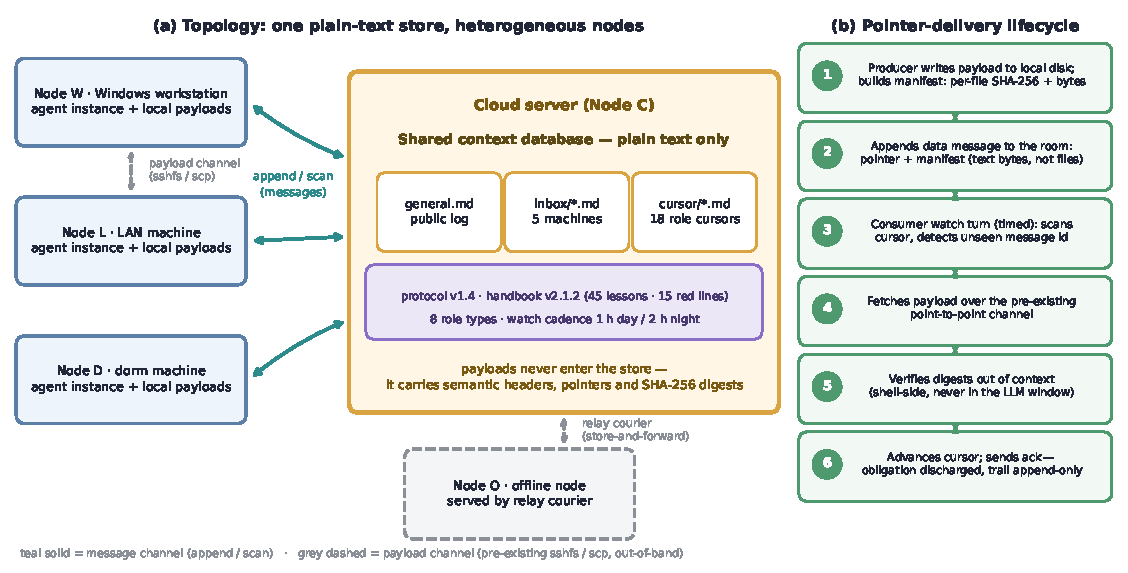
\includegraphics[width=\textwidth]{figures/fig1-overview.pdf}
\caption{\textbf{Figure 1.} Murmuration at a glance. (a) Heterogeneous
nodes coordinate through one shared plain-text store --- public log,
per-machine inboxes, per-role cursors --- under a versioned governance
handbook and time-triggered watchkeeping; payloads never enter the store
and move over pre-existing point-to-point channels. (b) Pointer-delivery
lifecycle: manifests and digests travel as text inside the context
budget; files are fetched out-of-band and verified shell-side.}
\end{figure*}



\section{Semantic-Level Transport Model}


\hypertarget{message-calculus}{%
\subsubsection{4.1 Message calculus}\label{message-calculus}}

\textbf{Definition 1 (semantic message).} A message is a triple
\(d = (a, p, r)\) where \(a\) is the \emph{act header} (performative
\(\pi \in \{\)ask, reply, note, data, ack\(\}\), identifier
\(\mathit{mid}\), unique per (producer, second), identity
\((m_{from}, \rho_{from}, m_{to})\) --- the sending machine and posting
role; the target role is resolved at delivery time from the addressed
inbox and is not carried on the wire --- a per-producer wall-clock
timestamp \(t\) with bounded (NTP-grade) skew, and an optional referent
\(re\)), \(p\) is an optional \emph{content-addressed pointer}
\((\text{path}, h, n)\) with \(h = \text{SHA-256}\) and byte count
\(n\), and \(r\) is an optional inline residue with \(|r| \le B\)
(deployment value \(B = 2\) KB).

\textbf{Definition 2 (channel).} A channel \(C\) is an append-only
sequence \(d_1, d_2, \dots\); its \emph{semantic projection} is the
sequence of headers and pointers only.

\textbf{Definition 3 (cursor).} For a consumer \((m, \rho)\), the cursor
\(\kappa(m,\rho)\) records the identifier --- and hence the embedded
fixed-width timestamp --- of its last consumed message; novelty is
decided by R3's suffix comparison against that timestamp. The cursor is
\emph{per consumer} (one file per machine--role pair) and is compared
against every channel the consumer scans (its inbox and the public
channel); it remains well-defined under partial replication (an offline
node's replica). One shared last-consumed identifier across two channels
can skip older messages in the second channel --- the cross-channel skip
hazard of §8 --- so consumers scan in a fixed channel order and accept a
residual window.

\textbf{Definition 4 (delivery manifest).} A delivery of payload set
\(P = \{f_1, \dots, f_k\}\) is one \texttt{data} message whose pointer
list enumerates \((\text{path}_i, h_i, n_i)\); acceptance requires, for
each \(i\), an out-of-context equality check
\(\text{SHA-256}(f_i) = h_i \land |f_i| = n_i\), after which the
receiver posts \texttt{ack}.

\textbf{Definition 5 (watch schedule).} A function
\(W: \text{time} \to \{\text{invoke}, \text{skip}\}\) re-invokes each
role on a cadence (deployment: 1 h daytime, 2 h night), implementing
time-triggered activation for agents that cannot listen.

\hypertarget{cost-model}{%
\subsubsection{4.2 Cost model}\label{cost-model}}

Let \(H\) be header+pointer size (hundreds of bytes) and \(|P|\) payload
size.

\textbf{Proposition 1 (context cost).} Assume manifests are generated
and digest-verified entirely out of context, with only per-file
boolean/summary lines entering it (the \emph{manifest assumption}; this
is exactly how the deployment's verification scripts run). Then the
context-window cost charged to sender and receiver for one delivery of
\(k\) files is \(O(k \cdot H)\), independent of payload bytes \(|P|\);
and when the pointer list itself exceeds the inline threshold it is
delivered as a file --- one pointer, \(O(H)\) --- restoring a constant
per-delivery context cost at any \(k\). \emph{Sketch.} By R4 the payload
never enters any context; only \(a\) and \(p\) do, plus the verifier's
summary. A manifest that is itself a payload is subject to R4 again,
which yields the two-case bound. \(\blacksquare\)

\textbf{Proposition 2 (O(1) novelty).} Given cursor \(\kappa\), and
assuming no two messages from the same producer share a timestamp second
(the uniqueness scope of \(\mathit{mid}\); §8(iv)), detecting whether
new messages exist costs one fixed-width string comparison per scanned
channel, not a scan of message bodies. \emph{Sketch.} Under that
uniqueness assumption, R3's suffix is a total order key; bodies are
irrelevant to novelty. \(\blacksquare\)

\textbf{Proposition 3 (relay idempotence).} Forwarding a pointer across
\(k\) hops charges \(O(H)\) context per hop, and the payload context is
paid zero times beyond the original posting: the pointer denotes the
same content at every hop, and verification remains end-to-end by digest
equality. \emph{Sketch.} Content addressing makes \(p\)
location-independent; under the standard assumption that SHA-256 is
collision-resistant, \(h\) ties pointer identity to content at every
hop. \(\blacksquare\)

These properties map directly onto the Multi-Agent System Failure
Taxonomy (MAST) {[}13{]}: specification ambiguity is bounded by five
performatives with mandatory referents; inter-agent misalignment is
bounded by explicit ack obligations (§5); unrecoverable failures become
visible because every act is logged append-only; and context
poisoning/overflow is bounded by Proposition 1. We state this as
\emph{design intent}, not as measured efficacy; incident-level grounding
(incident → patching rule) ships as a repository artifact (§6).

\hypertarget{lineage}{%
\subsubsection{4.3 Lineage}\label{lineage}}

Speech acts {[}14{]} → KQML {[}15{]} → FIPA-ACL {[}16{]} supply the
performative discipline; Linda and blackboards {[}17,18{]} supply shared
coordination artifacts; publish/subscribe with consumer offsets (Kafka
logs) {[}19,20{]} supply cursors; Merkle trees and IPFS content
addressing {[}21,22{]} and W3C PROV {[}23{]} supply pointers and
provenance; event- versus time-triggered architecture {[}24{]} supplies
the watch schedule; goal-oriented semantic communication {[}25,26{]}
supplies the ``transmit intent, not bits'' stance; and stigmergy
{[}27{]} and coordination theory {[}28{]} frame the room itself as an
indirect-coordination medium. Classical ACL protocols assume that
receiving is cheap: content travels inline and receiver cost is the
sender's concern. Murmuration inherits their performative discipline but
inverts the cost model for context-bounded receivers --- payload bytes
are replaced by content-addressed pointers verified outside context, and
the R4 threshold caps what any single header can charge a receiver's
window. Which discipline is inherited and which constraint is new is
exactly the distinction the L2 claim (§7) rests on. The combination ---
and its reduction to \emph{plain files} as the universal narrow waist
--- is what we contribute.



\section{Organizational Governance}


Transport without governance decays: roles blur, obligations lapse,
lessons evaporate. Murmuration specifies four instruments, in the
tradition of electronic institutions and organizational design for MAS
{[}29,30{]}.

\textbf{Roles.} Named posts per machine (diplomat, mechanic, editor,
coordinator, \ldots{}); a machine may hold several; every message header
carries the posting role, making responsibility auditable.

\textbf{Versioned handbook with red lines.} Cross-machine lessons live
in an append-only handbook with numbered entries and an index;
operational prohibitions are \emph{red lines} with monotonic numbering
(never renumbered). Crucially, red lines are \textbf{incident-driven
patches}: each of the 13 archived incidents from the deployment history
(one predating the study window) produced at least one rule (e.g., a
session-registry overwrite incident produced the ``never rewrite
coordination state'' family; a tunnel-death incident produced the
watchdog rule). The handbook is thus a living patch series over the
organization's failure surface.

\textbf{Acknowledgment obligations.} Borrowing from commitment-based MAS
semantics {[}31{]}: a \texttt{data} or \texttt{ask} message creates a
debtor obligation on its addressee, discharged only by \texttt{ack} or
\texttt{reply}. A derived \textbf{ack board} (two columns: inbound
obligations uncleared; outbound messages awaiting discharge) is
computable from the logs alone and drives the watch turns.

\textbf{Time-triggered watchkeeping.} Because agents cannot block
(Definition 5), liveness is a schedule. Cadence is a policy parameter
(day/night tiers), and each watch turn is a fixed checklist: scan
cursors, discharge obligations, update the board, escalate staleness.

\textbf{Recovery.} All organizational state is rebuildable from the logs
alone. A lost or corrupted cursor is repaired by rescanning its channel
from the first message and re-deriving the last-consumed identifier; the
duplicate re-dispatch this may cause is harmless because acknowledgment
discharge is idempotent per referent (an \texttt{ack} naming an
already-discharged \texttt{mid} is a no-op), so recovery costs one
linear scan and never payload re-verification unless a digest is
re-challenged. A restarted watcher resumes from its cursor file; if that
file is missing too, it adopts the channel tail only after posting a
human-visible \texttt{note} announcing the reset, so the operator can
veto silent state loss.



\section{Field Study (sanitized)}


Five heterogeneous machines (a Windows workstation, a cloud Linux server
hosting the shared database, a LAN node, a dormitory node, and an
offline node served by relay) ran the method for eleven elapsed days
(2026-10-22 → 11-02; twelve calendar days inclusive). Machine names are
pseudonyms; all identifiers, paths, and contents are sanitized.

\begin{itemize}
\tightlist
\item
  \textbf{Protocol evolution:} v1.0 → v1.4 within the eleven-day window,
  all changes backward-compatible; each minor version traceable to
  incidents or onboarding friction.
\item
  \textbf{Organization:} eight role types; multi-role machines; one
  editor-in-chief owns the shared handbook (v2.1.2: four volumes, 45
  cross-machine lessons, 15 red lines, 13 incident archives).
\item
  \textbf{Deliveries:} thousand-file-scale packages (chapter drafts,
  figure sets, CSV matrices) moved as pointer manifests with per-file
  SHA-256 + byte verification --- a corruption check, not an
  authenticity control (§8); zero digest mismatches across all verified
  files; per-delivery context cost stayed at header scale in operator
  observation (not separately metered).
\item
  \textbf{Volume (sanitized counts only):} 283 structured messages
  across one public channel, five machine inboxes and eighteen role
  cursors during the window (mean 26/day, peak 49/day); 37 \texttt{data}
  deliveries, 29 \texttt{ask}s, 89 \texttt{ack}/\texttt{reply}
  discharges, 120 status notes, and 8 governance posts (four notices, a
  request, an action marker, a report, a correction); more than three
  thousand per-file SHA-256 digests checked with byte equality in total,
  largest single manifest above 1,300 files.
\item
  \textbf{Task classes (abstracted):} scientific-experiment data
  pipelines, long-form document drafting, and paper writing; no payload
  content is disclosed --- only counts, shapes and verification
  outcomes.
\item
  \textbf{Liveness:} watch cadence institutionalized (1 h day / 2 h
  night); a 48-hour escalation rule for unanswered obligations; weekly
  digest.
\item
  \textbf{Failure pedagogy:} the room rules R2, R3, and R5 each exist
  because a real message was lost or misordered without them; a related
  message-fence parsing rule was adopted later (2026-11-08) from a local
  smoke-test regression outside the study window and never caused a
  room-level loss.
\end{itemize}

\textbf{A natural ablation.} Because every rule is a patch for a
recorded incident, the deployment history is a natural ablation: each
rule partitions the timeline into a before-period with an observed
failure and an after-period without recurrence. In the window, the
incident-derived room rules (R2, R3, R5) showed no recurrence after
adoption, and no incident recurred after its ops red line (the
machine-layer rule family, numbered separately from the room rules) was
written; per-rule exposure denominators are not separately metered, so
these are narrative, not causal, claims. The full counterfactual tables
and honesty caveats ship as a repository artifact
(\texttt{docs/research/natural-ablation.md}).

\begin{figure*}
\centering
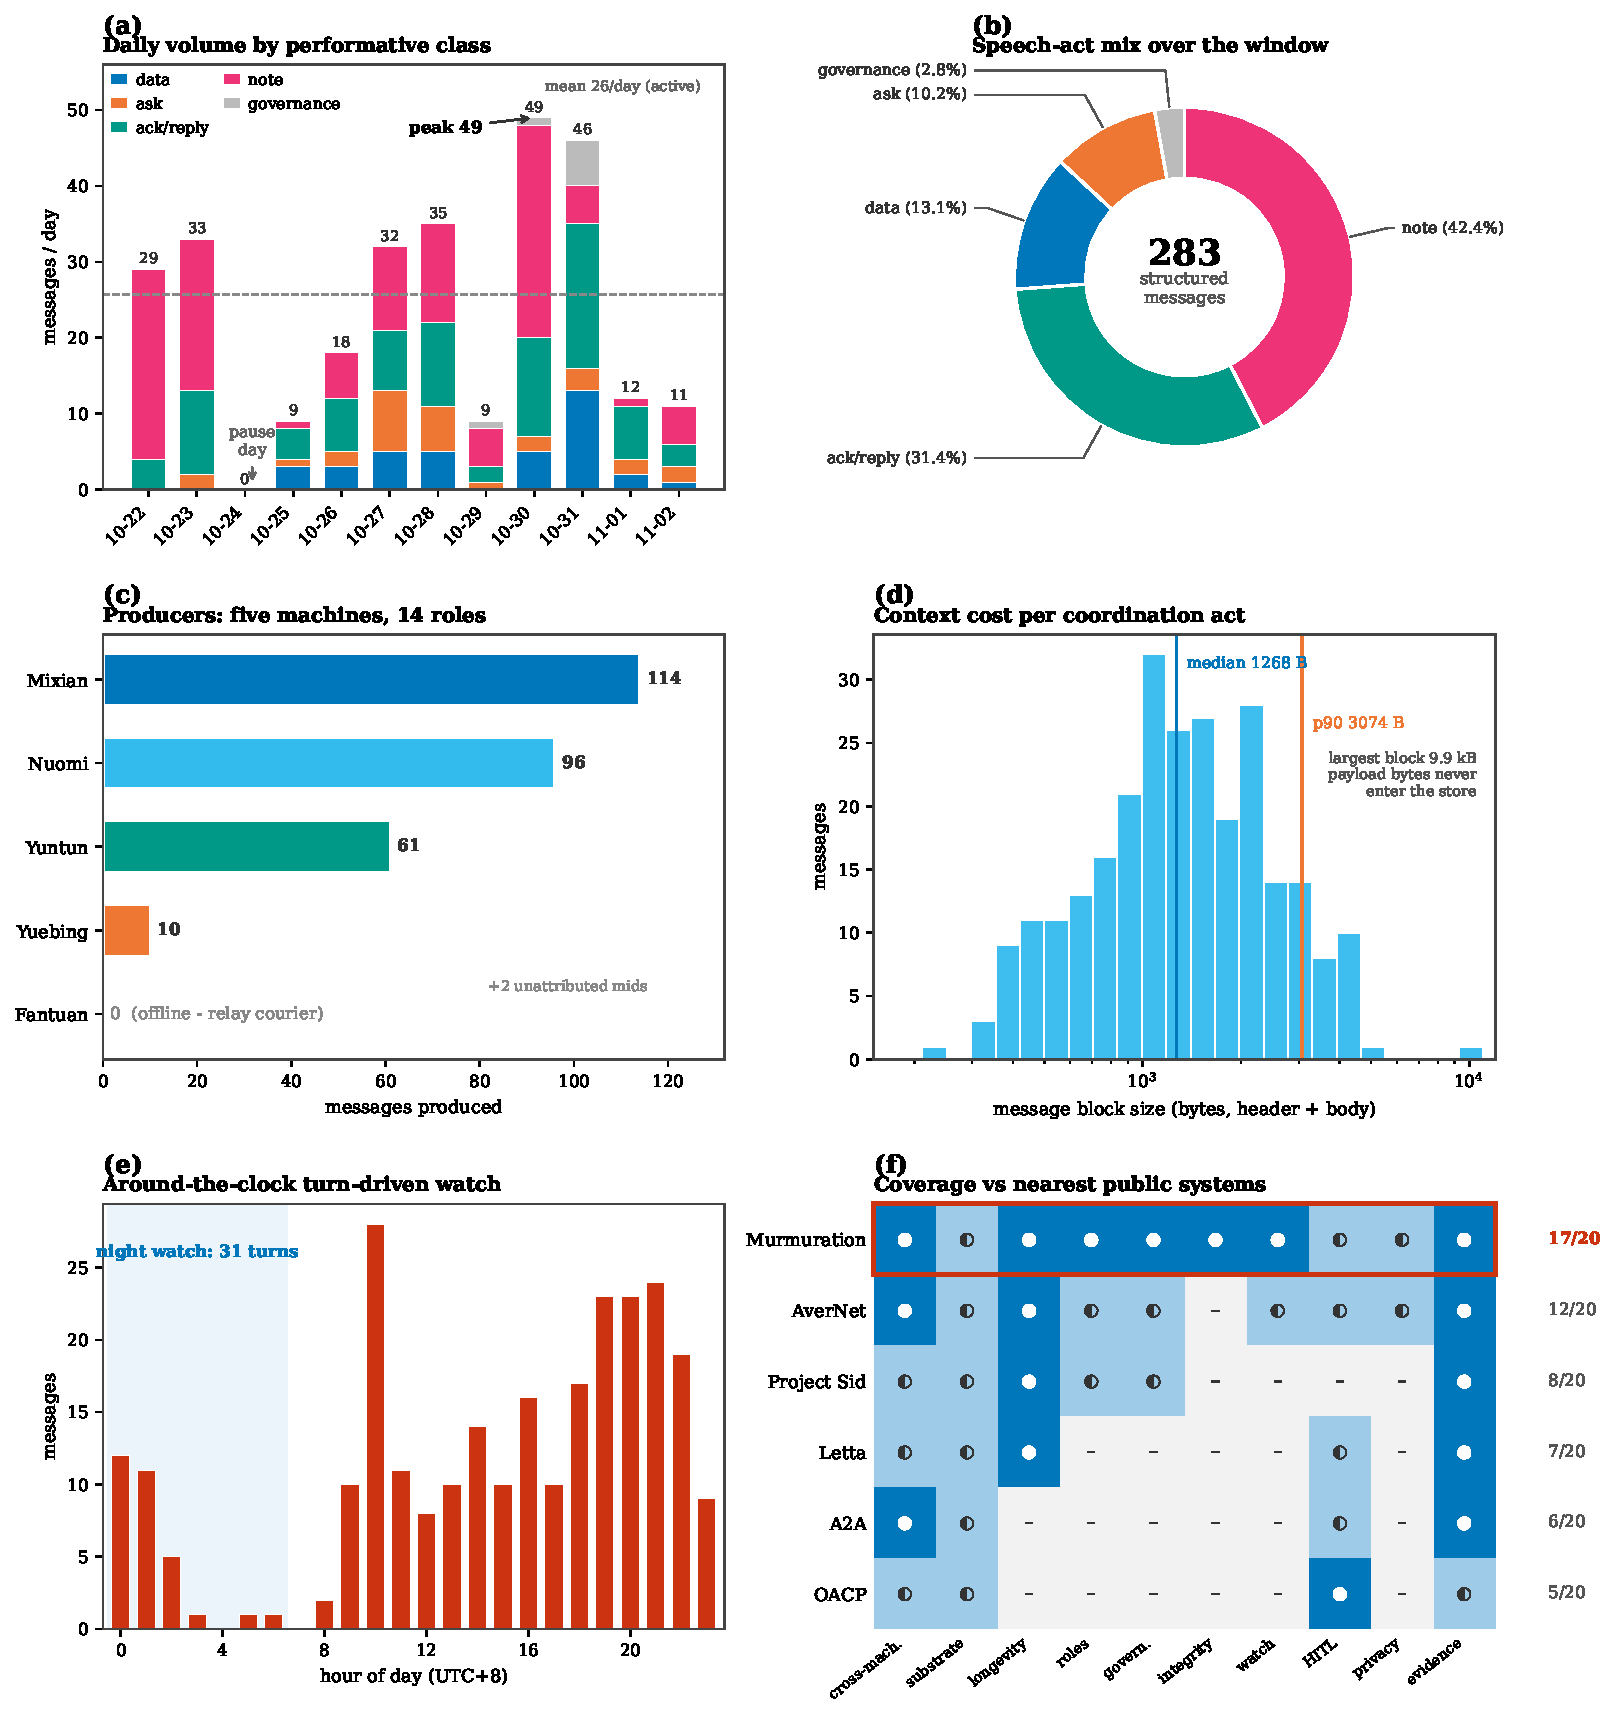
\includegraphics[width=\textwidth]{figures/fig2-field-dashboard.pdf}
\caption{\textbf{Field-study dashboard over the census window} (five
machines, 2026-10-22 to 2026-11-02). \textbf{(a)} Daily
structured-message volume by performative class (\(n=283\)); mean 26/day
over active days, peak 49 on Oct 30; the pause day saw no posts.
\textbf{(b)} Speech-act mix: 37 data deliveries, 29 asks, 89 ack/reply
discharges, 120 notes, and 8 governance posts. \textbf{(c)} Producers by
machine; the fifth machine ran offline and was served by a relay
courier. \textbf{(d)} Message block sizes (\(n=265\) parsed blocks, log
scale): coordination acts cost hundreds of bytes of context, while
payload bytes move out-of-band. \textbf{(e)} Arrival-hour profile: 31
turns occurred in the 00:00-07:00 night window under turn-driven
watchkeeping. \textbf{(f)} Coverage across the ten dimensions of Section
7 for the five nearest public systems (filled circle = full, half circle
= partial, dash = absent); scores are dimension sums.}
\end{figure*}

We report this as \emph{existence evidence} for operability, not as a
controlled evaluation.

\textbf{A controlled ablation (2026-11-09).} To separate the contribution of the coordination substrate from task or model effects, we ran a controlled A0-vs-A1 ablation: six abstracted tasks, three rounds each, executed by the same model and harness either as a single session (A0) or as a two-agent federation over the room protocol (A1), in one continuous time window with a Latin-square arm order (R1 A0 first, R2 A1 first, R3 A0 first). All 36 runs completed with zero human interventions and zero runner fallback; every artifact passed verification on first attempt (18/18 per arm). The federation arm cut makespan by 34\% (215.0~s to 141.7~s per round, $1.52\times$; lower in every round, with three-times-lower range variance), at the price of $+1.3$ turns and $+57\%$ context bytes per task ($1{,}908$ to $2{,}992$~B, dominated by room-pointer reads of $1{,}439$~B per task against a $\approx$2~KB payload). The pointer overhead is payload-scale-dependent, so the economy argument of Section~4 remains open for larger payloads; verification quality was parity (first pass 18/18 in both arms). With $n=3$ rounds we claim no significance; per-round numbers and the byte-class breakdown ship as a repository artifact (\texttt{docs/experiments/ablation-results/}).

\begin{figure*}
\centering
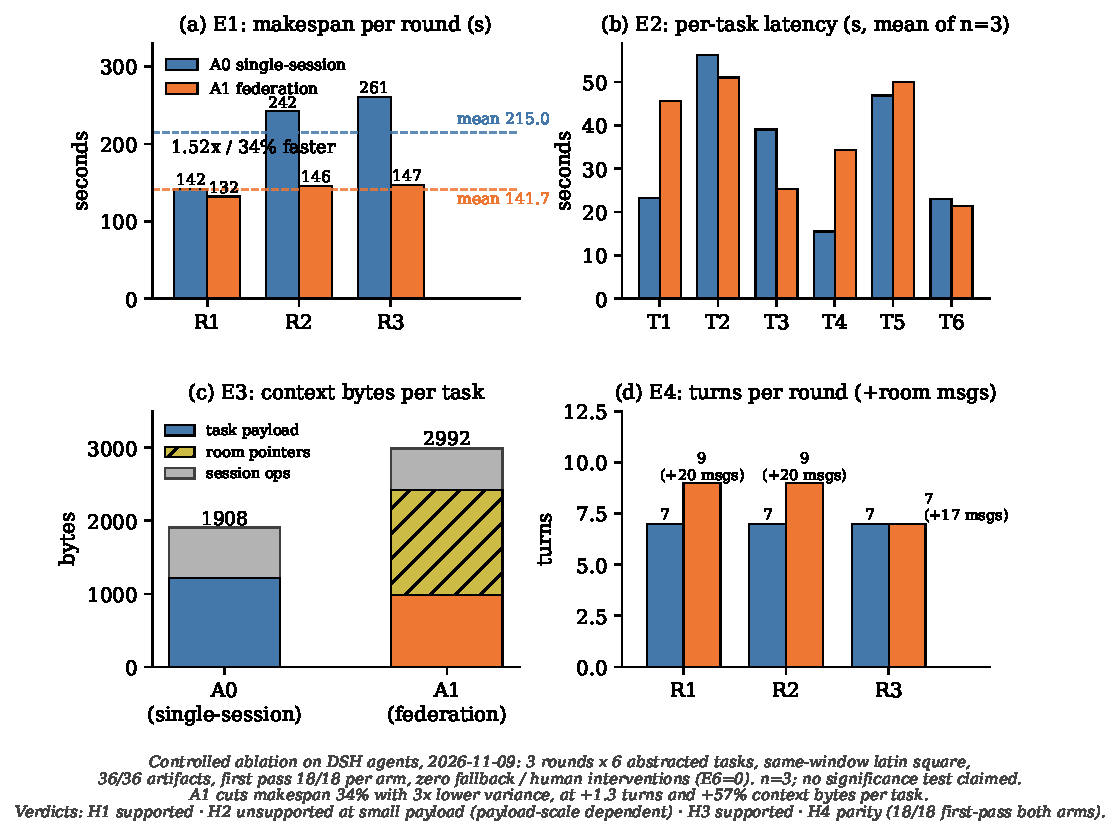
\includegraphics[width=\textwidth]{figures/fig3-ablation.pdf}
\caption{\textbf{Controlled ablation, A0 single-session vs.\ A1 room-federated} (same-window Latin square, $n=3$; zero interventions, zero fallback). \textbf{(a)} E1: makespan per round; A1 is lower in every round (means 141.7 vs.\ 215.0~s, $1.52\times$ / 34\% faster, 3$\times$ lower variance). \textbf{(b)} E2: per-task latency (mean of $n=3$); A1 includes room-acknowledgment queueing. \textbf{(c)} E3: context bytes read per task by class; A1's pointer reads (1,439~B/task) exceed its payload saving at this $\approx$2~KB payload scale, so H2 (context economy) is unsupported at small payloads. \textbf{(d)} E4: turns per round with room-message counts; the federation pays $+1.3$ turns and 57 room messages (H3, coordination overhead, supported). Verification parity: first pass 18/18 per arm (H4). No significance test is claimed at $n=3$.}
\end{figure*}

\textbf{Artifact availability.} The framework source, plugin tools, and
the research artifacts behind §7 --- the 49-system × 10-dimension
novelty matrix, the search log, the adversarial re-review, and the claim
ladder --- ship in the public repository accompanying this paper
(github.com/xuanjat/murmuration, under \texttt{docs/research/} and \texttt{docs/experiments/});
documentation is licensed CC BY 4.0.



\section{Novelty Assessment and Claim Ladder}


We compared 49 systems across 10 dimensions --- (1)
cross-machine/network topology, (2) coordination substrate, (3)
longevity (persistent organization vs.~single task), (4) role systems
including multi-role machines, (5) governance mechanisms, (6)
delivery-integrity protocols, (7) watchkeeping/wake-up models, (8)
human-in-the-loop boundaries, (9) privacy-boundary discipline, and (10)
real operational evidence --- spanning single-host orchestrators,
cross-machine protocols, Claude/DSH-ecosystem tools, memory systems,
academic simulations, and governance toolkits; the full matrix, search
log, and adversarial re-review ship as repository artifacts.

Nearest neighbors: (a) \textbf{Avernet} {[}11{]}, a platform substrate
for organization-scale persistent agents
(identity/discovery/routing/containers; since 2026-09 it also ships a
DSH channel plugin) --- a different route: the distinction is
administrative footprint and auditability, not the presence of
infrastructure --- the shared store is itself a hosted database service,
but one append-only text store is a far lighter administrative footprint
than identity, discovery, routing, and container orchestration, and
every coordination artifact remains human-readable; (b) \textbf{ruflo}
(formerly claude-flow) {[}8{]}, a single-box swarm framework with
hierarchical memory --- complementary, not cross-machine; (c)
\textbf{built-in single-host agent teams} {[}9{]} and conversation-based
orchestrators {[}5,6,7{]} --- complementary; (d) \textbf{concurrent
single-organization super-agent architecture} (two-layer Router/Worker,
event triggers with thread subscription, Inline \& Spill and
Chain-of-Recall context mechanics, Watchdog control loop; prototype
plugin \texttt{dsh-superagent-prototype}) {[}12{]} --- same motivation
(attention bottleneck, session silos), different unit of redesign: they
re-engineer one organization's agent interior with programmatic routing
and push events on a single harness deployment, whereas we leave every
instance untouched and add only a cross-instance organizational layer
that works across machines and harness builds; their stated open
problems (A2A between agent instances, collaboration detached from
sessions) are precisely the surfaces our room protocol, pointer
delivery, and ack obligations specify. Cross-machine agent protocols
such as A2A {[}10{]} standardize task exchange between reachable service
endpoints but do not specify governance, delivery integrity, or
watchkeeping for turn-based personal instances behind NAT or on offline
links. (e) Per-element closest neighbors from the repository matrix:
cross-machine topologies --- Avernet {[}11{]}, IoA, AgentScope, ANP, A2A
(all presuppose service endpoints or online connectivity);
shared-substrate coordination --- Letta's shared memory blocks and the
mcp-agent-mail shared inbox (single-host; no delivery-integrity
protocol); governance --- a policy/compliance governance toolkit and
academic institutional design (no versioned, incident-driven handbook
evolution); delivery integrity --- governance-toolkit audit trails
(closest neighbor, but a different purpose: retrospective compliance
logging, not receiver-side acceptance); watchkeeping --- night-shift
batch schedulers and cron-style wake-ups (scripts, no persistent
organization or ack obligations); field evidence --- simulation studies
such as Project Sid (not a deployment).

Per our search (2026-11), no public scheme combines heterogeneous
cross-machine instances + a shared plain-text context database as the
sole substrate (in this design) + versioned incident-driven handbook
governance + pointer-based delivery-integrity protocol + turn-driven
time-triggered watchkeeping + field evidence. Our claim ladder --- a
repository discipline with an explicit weakest-to-strongest ordering: L0
(unqualified ``first-ever'' claims) and L1 (``first open-source''
claims) are forbidden as unverifiable by exhaustive search, L2
(qualified combination novelty) is the ceiling this paper uses, L3
(contribution statements without uniqueness) fills the contributions
list, and L4 (reusability-only) is the retreat position under challenge
--- states results at level L2 (``combination unseen in search'') with
contribution-style L3 sentences; ``first-ever'' claims are explicitly
disclaimed, and the strongest single dimension is delivery integrity
(dimension 6: digest discipline outside context), the weakest are
cross-machine topology (dimension 1: every surveyed scheme already
federates machines in some form) and human-in-the-loop boundaries
(dimension 8: standard interrupt/approval support).



\section{Limitations}


No push delivery (polling only); no server-side deduplication or
permission isolation in the substrate (compensated by cursor discipline
and red lines); a single shared trust root; parameters (2 KB, cadences)
are deployment choices, not optima; metrics are self-reported from one
organization; the MAST alignment is design intent, not measured
efficacy; the comparison with concurrent super-agent designs {[}12{]} is
qualitative --- their measurements run on synthetic loads, ours on
sanitized field logs, and no head-to-head benchmark exists.

\textbf{Distributed-systems candor.} (i) \emph{Concurrent appends:} R1's
history guarantee assumes appends do not interleave; network filesystems
generally provide neither atomic append nor locking. The deployment
compensates with role discipline (per-machine files, diplomat-mediated
posting to the public channel) --- discipline, not a filesystem
guarantee. The substrate's per-append atomicity is in fact what the
safety argument leans on: inboxes remain writable by any machine, so
acknowledgment fan-in from many receivers to one inbox is serialized
only by that property, and §3's history guarantee is conditional on it.
(ii) \emph{Integrity versus authenticity:} SHA-256 digests detect
corruption, not adversarial substitution; any writer with substrate
access could replace a payload and recompute its digest. The threat
model of §2 presumes a single, mutually trusted trust root. (iii)
\emph{Injection bus:} message bodies enter peers' contexts verbatim, so
a compromised node could attempt to steer the others; current
mitigations are procedural (red lines, human-auditable plain text), not
a data/instruction separation mechanism --- an open problem for LLM
federations generally. (iv) \emph{Clocks and collisions:} R3's ordering
presumes bounded (NTP-grade) clock skew across machines, and
seconds-granular \texttt{mid}s can still collide for two same-second
messages from one (machine, role). (v) \emph{Relay consistency:} replica
merging and duplicate handling for offline nodes rest on cursor
discipline, without a formal reconciliation protocol. (vi)
\emph{Unbounded growth:} append-only logs have no archival or
garbage-collection policy; watch-turn scans grow with the log. (vii)
\emph{Liveness bound:} worst-case obligation latency is the watch
cadence plus the 48-hour escalation window; nothing tighter is
guaranteed. (viii) \emph{Cursor races and channel skips:} a cursor file
is read, compared, and rewritten by its owner, and two concurrent watch
turns of the same role can race on that read-modify-write --- mitigated
by one-file-per-role and turn scheduling, not eliminated; the single
cursor also spans both channels a role scans, so advancing it on one
channel can silently skip older messages on the other (the cross-channel
skip hazard of Definition 3), narrowed by fixed channel order. (ix)
\emph{Parsing fragility:} message boundary detection depends on fence
handling; a substrate append that drops a trailing newline can glue the
next header into the previous body --- the 2026-11-08 local regression
behind the message-fence parsing rule (§6), mitigated by blank-line
padding and read-back self-checks. (x) \emph{Offline clock discipline:}
the relay-served offline node's clock is not NTP-disciplined, so its
messages can be judged stale by R3 comparisons; the skew assumption of
(iv) is unverified for that node.



\section{Conclusion}


Murmuration suggests that a federation of independent, heterogeneous LLM
agents can be coordinated in the coordination plane with \emph{nothing
but text} --- payload bytes move over pre-existing point-to-point
channels (§2): semantic headers and content-addressed pointers keep the
scarce resource --- context --- free of payloads, while a versioned
handbook, ack obligations, and time-triggered watchkeeping keep the
organization alive between turns. The eleven-day, five-machine
deployment indicates that the design is not merely implementable on
paper but operable in sustained use, and its incident-driven rule set is
a reusable artifact for anyone running personal agent federations.




\begin{thebibliography}{31}

\bibitem{r1}
Guo, T., et al. (2024). Large language model based multi-agents: a survey of progress and challenges. \emph{arXiv:2402.01680} (IJCAI 2024).

\bibitem{r2}
Zhang, Z., et al. (2024). A survey on the memory mechanism of large language model based agents. \emph{arXiv:2404.13501}.

\bibitem{r3}
Liu, N. F., et al. (2024). Lost in the middle: how language models use long contexts. \emph{TACL} (arXiv:2307.03172).

\bibitem{r4}
Chen, L., Zaharia, M., \& Zou, J. (2023). FrugalGPT: how to use large language models while reducing cost and improving performance. \emph{arXiv:2305.05176}.

\bibitem{r5}
Wu, Q., et al. (2023). AutoGen: enabling next-gen LLM applications via multi-agent conversation. \emph{arXiv:2308.08155}.

\bibitem{r6}
Hong, S., et al. (2023). MetaGPT: meta programming for a multi-agent collaborative framework. \emph{arXiv:2308.00352}.

\bibitem{r7}
Qian, C., et al. (2023). Communicative agents for software development. \emph{arXiv:2307.07924}.

\bibitem{r8}
ruflo (formerly claude-flow) (2026). \emph{Single-box agent swarm orchestration with hierarchical memory}. https://github.com/ruvnet/ruflo (repository, accessed 2026-11).

\bibitem{r9}
DeepSeek (2026). \emph{DeepSeek Harness (DSH)} --- a local-first LLM-agent harness with built-in single-host Agent Teams --- and \emph{OpenViking}, its shared context database. npm package \texttt{@deepseek-ai/dsh}: https://www.npmjs.com/package/@deepseek-ai/dsh (accessed 2026-11).

\bibitem{r10}
Linux Foundation (2025). \emph{Agent2Agent (A2A) protocol specification}.

\bibitem{r11}
inclusionAI (2026). \emph{Avernet: infrastructure for persistent, organization-scale multi-agent systems}. https://github.com/inclusionAI/Avernet (repository documentation, accessed 2026-11).

\bibitem{r12}
DeepSeek Harness Team (2026). \emph{Super-agent design exploration: toward more autonomous agent systems} (in Chinese) (architecture exploration article, 2026-11-01; prototype: dsh-superagent-prototype). Coverage: DoNews, https://www.donews.com/news/detail/1/6760986.html; PChome, https://article.pchome.net/news/16524.html (both 2026-11-01).

\bibitem{r13}
Cemri, M., et al. (2025). Why do multi-agent LLM systems fail? \emph{arXiv:2503.13657} (NeurIPS 2025 Datasets \& Benchmarks).

\bibitem{r14}
Searle, J. R. (1969). \emph{Speech Acts: An Essay in the Philosophy of Language}. Cambridge University Press.

\bibitem{r15}
Finin, T., Fritzson, R., McKay, D., \& McEntire, R. (1994). KQML as an agent communication language. In \emph{Proceedings of CIKM '94}. ACM.

\bibitem{r16}
FIPA (2002). \emph{FIPA Communicative Act Library Specification}, document no. SC00037F. Foundation for Intelligent Physical Agents. http://www.fipa.org/specs/fipa00037/.

\bibitem{r17}
Gelernter, D. (1985). Generative communication in Linda. \emph{ACM TOPLAS}, 7(1).

\bibitem{r18}
Nii, H. P. (1986). Blackboard systems. \emph{AI Magazine}, 7(2).

\bibitem{r19}
Eugster, P. Th., Felber, P. A., Guerraoui, R., \& Kermarrec, A.-M. (2003). The many faces of publish/subscribe. \emph{ACM Computing Surveys}, 35(2).

\bibitem{r20}
Kreps, J., Narkhede, N., \& Rao, J. (2011). Kafka: a distributed messaging system for log processing. \emph{NetDB '11}.

\bibitem{r21}
Merkle, R. C. (1980). Protocols for public key cryptosystems. \emph{IEEE Symposium on Security and Privacy}.

\bibitem{r22}
Benet, J. (2014). IPFS --- content addressed, versioned, P2P file system. \emph{arXiv:1407.3561}.

\bibitem{r23}
Moreau, L., et al. (2013). \emph{PROV-Overview: An Overview of the PROV Family of Documents}. W3C.

\bibitem{r24}
Kopetz, H. (1991). Event-triggered versus time-triggered real-time systems. In \emph{Operating Systems of the 90s and Beyond} (Dagstuhl Seminar), LNCS 563. Springer.

\bibitem{r25}
Shannon, C. E., \& Weaver, W. (1949). \emph{The Mathematical Theory of Communication}. University of Illinois Press.

\bibitem{r26}
Luo, J., Delfani, E., Salimnejad, M., \& Pappas, N. (2025). From information freshness to semantics of information and goal-oriented communications. \emph{arXiv:2512.12758}.

\bibitem{r27}
Theraulaz, G., \& Bonabeau, E. (1999). A brief history of stigmergy. \emph{Artificial Life}, 5(2).

\bibitem{r28}
Malone, T. W., \& Crowston, K. (1994). The interdisciplinary study of coordination. \emph{ACM Computing Surveys}, 26(1).

\bibitem{r29}
Esteva, M., Rodríguez-Aguilar, J. A., Sierra, C., García, P., \& Arcos, J. L. (2001). On the formal specification of electronic institutions. \emph{AMEC III}, Springer.

\bibitem{r30}
Hübner, J. F., Sichman, J. S., \& Boissier, O. (2007). Moise+: towards a structural, functional, and deontic model for multi-agent organizations. \emph{International Journal of Agent-Oriented Software Engineering}, 1(3/4).

\bibitem{r31}
Singh, M. P. (1999). An ontology for commitments in multiagent systems. \emph{Artificial Intelligence and Law}, 7(1). 

\end{thebibliography}

\end{document}
